\chapter{Estado de la Cuestión}
\label{cap:estadoDeLaCuestion}

En el estado de la cuestión es donde aparecen gran parte de las referencias bibliográficas del trabajo. Una de las formas más cómodas de gestionar la bibliografía en {\LaTeX} es utilizando \textbf{bibtex}. Las entradas bibliográficas deben estar en un fichero con extensión \textit{.bib} (con esta plantilla se proporciona el fichero biblio.bib, donde están las entradas referenciadas más abajo). Cada entrada bibliográfica tiene una clave que permite referenciarla desde cualquier parte del texto con los siguiente comandos:

\begin{itemize}
\item Referencia bibliografica con cite: \cite{ldesc2e}
\item Referencia bibliográfica con citep: \citep{notsoshort}
\item Referencia bibliográfica con citet: \citet{latexAPrimer}
\end{itemize}

Es posible citar más de una fuente, como por ejemplo \citep{latexCompanion,LaTeXLamport,texKnuth}

Después, latex se ocupa de rellenar la sección de bibliografía con las entradas \textbf{que hayan sido citadas} (es decir, no con todas las entradas que hay en el .bib, sino sólo con aquellas que se hayan citado en alguna parte del texto).

Bibtex es un programa separado de latex, pdflatex o cualquier otra cosa que se use para compilar los .tex, de manera que para que se rellene correctamente la sección de bibliografía es necesario compilar primero el trabajo (a veces es necesario compilarlo dos veces), compilar después con bibtex, y volver a compilar otra vez el trabajo (de nuevo, puede ser necesario compilarlo dos veces). 


\section{Cuestiones básicas de inmunología}

Antes de comenzar sería conveniente introducir una serie de términos básicos referentes al sistema inmune. De esta manera los conceptos y modelos que se expondrán más adelante serán entendidos sin ningún impedimento terminológico. 

\subsection{El sistema inmune innato}
Como ya hemos comentado en la sección \ref{cap:introduccion} de Introducción, el sistema inmune funciona como un equipo. Está compuesto por numerosas células, proteínas y otros agentes de distinto tipo que trabajan de forma coordinada para dar una respuesta eficaz y proporcional al ataque recibido. Pero comencemos por lo más simple: las barreras físicas. La piel y la mucosa de nuestro sistema respiratorio, digestivo y reproductivo intentan que virus, bacterias, hongos o parásitos entren en nuestro organismo. Pero, ¿qué pasa si estos logran atravesar esta barrera?

Aquí entra lo que se denomina \textit{sistema inmune innato}, este recibe este nombre porque parece la defensa ``natural'' que todo animal parece tener. De hecho, muchos mecanismos de este sistema inmune innato llevan con nosotros más de 500 millones de años. 
Entre los jugadores más famosos de este equipo encontramos los \textit{macrófagos}. Su nombre compuesto por ``macro'', que significa grande y ``fago'', que viene del Griego y significa comer, lo dice todo. En efecto, los macrófagos son células que se comen invasores mediante un proceso llamado \textit{fagocitosis}, que ilustra la figura \ref{fig:macrofago}.


\begin{figure}[t]
	\centering
	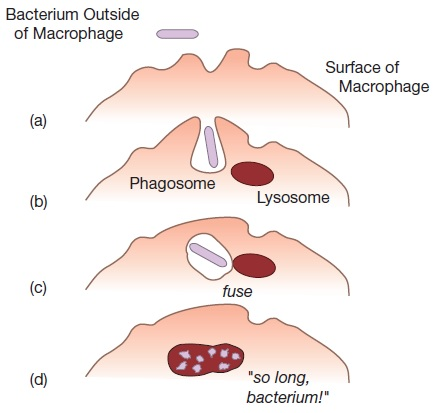
\includegraphics[width=0.5\textwidth]{1_macrofago}
	\caption{Fagocitación de un macrófago a una bacteria.}
	\label{fig:macrofago}
\end{figure}


Durante la batalla, los \textit{macrófagos} producen y secretan unas proteínas llamadas \textit{citoquinas}.
Estas son hormonas que facilitan la comunicación entre células del SI y cobrarán un papel muy relevante en los capítulos que siguen.
Podríamos decir que los \textit{macrófagos} hacen el papel de centinelas, que cuando ven al enemigo mandan señales (\textit{citoquinas}) para reclutar a más defensores.

\subsection{El sistema inmune adaptativo}

Los \textit{macrófagos} son células muy importantes del SI, pero no son las únicas. Durante nuestra andanza por este preámbulo al mundo inmunológico veremos otros tipos de células, en este caso referentes al \textit{sistema inmune adaptativo}.

El nombre es bastante descriptivo y, valga la redundancia, gracias a este SI somos capaces de adaptar nuestras defensas contra nuevos invasores.

CONTAR EJ COWPOX???????????

Seguro que el término \textit{anticuerpo} no resulta desconocido, pero ¿a qué nos referimos con él? Los \textit{anticuerpos} no son más que proteínas especiales que circulan por la sangre, y el agente que las produce se denomina \textit{antígeno}. Gracias a su estructura, los \textit{anticuerpos} son capaces de encajar en un determinado \textit{antígeno}. Cada \textit{anticuerpo} es producido por células B. Este tipo de células empiezan con el mismo ADN, pero cuando empiezan a madurar el ADN que forma los anticuerpos puede cambiar. Dando lugar así a gran diversidad de ellos y permitiendo la adaptabilidad de nuestro SI.

La misión principal de los \textit{anticuerpos} es identificar a los ``indeseables'', dejando que el trabajo sucio lo hagan otros. Es decir, gracias a la presencia de \textit{anticuerpos}, otras células, como los ya conocidos \textit{macrófagos} son capaces de identificar a los atacantes. Esto se ilustra en la figura \ref{fig:macrofago_anticuerpo}

\begin{figure}[t]
	\centering
	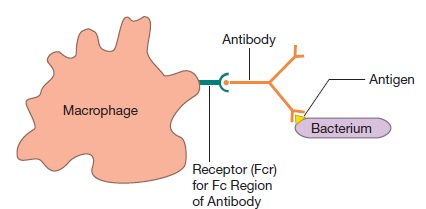
\includegraphics[width=0.5\textwidth]{2_macrofago_anticuerpo}
	\caption{Macrófago reconociendo una bacteria gracias a la acción anticuerpo-antígeno.}
	\label{fig:macrofago_anticuerpo}
\end{figure}

Aunque los \textit{anticuerpos} puedan ayuden a identificar a los malos, ¿qué ocurre cuando un virus ya ha entrado en una célula de nuestro cuerpo?. Los \textit{anticuerpos} no pueden alcanzarlo y el virus puede dedicarse a replicarse cuanto quiera. En este momento, es el turno de las células T. 

 